\documentclass[16 pt]{amsart}
\usepackage{amscd,amsmath,amsthm,amssymb}
\usepackage{enumerate,varioref}
\usepackage{epsfig}
\usepackage{graphicx}
\usepackage{mathtools}
\usepackage{tikz}
\usepackage{amsfonts}
\usepackage{svg}
\usetikzlibrary{graphs,arrows,topaths}
\newtheorem{thm}{Theorem}
\newtheorem{cor}[thm]{Corollary}
\newtheorem{lem}[thm]{Lemma}
\newtheorem{prop}[thm]{Proposition}
\theoremstyle{definition}
\newtheorem{defn}[thm]{Definition}
\theoremstyle{remark}
\newtheorem{ex}[thm]{Example}
\newtheorem{rem}[thm]{Remark}
\numberwithin{equation}{subsection}
\newcommand{\R}{\mathbb{R}}
\newcommand{\Z}{\mathbb{Z}}
\newcommand{\C}{\mathbb{C}}
\newcommand{\Q}{\mathbb{Q}}
\newcommand{\trail}[3]{a e_{#1} b e_{#2} a e_{#3} b e_5 c }
\begin{document}

\title{Homework 5 Maths 140 Winter 2015}
\maketitle 

10.3.11:Give an example of two matrices $A,B$ so that $AB \neq BA$

\vspace{1in}

Solution: Almost any two matrices will work here.  The easiest examples are those of nonsquare matrices.  Consider for example a matrix $A$ which is $n\times k$ and a matrix $B$ which is $k\times n$. Then the product $AB$ is $n\times n$ and $BA$ is $k\times k$.  They are not even the same size.  Much less the same matrix.  For a concrete example consider
\[
A = \begin{bmatrix}
1 & 2 \\ 3& 4
\end{bmatrix}
, B = \begin{bmatrix}
0 & 1 \\ 1 & 0
\end{bmatrix}
\]

Then 
\[
AB = \begin{bmatrix}
2 & 1 \\ 4 & 3
\end{bmatrix} 
\text{ and } 
BA = \begin{bmatrix}
3 & 4 \\ 1 & 2
\end{bmatrix}
\]

We see that $B$ switches columns when it is on the right, but switches rows when it is on the left.

\newpage

10.3.12: Let $O$ be the zero matrix Find two $2\times 2$ matrices $A,B$ so that $A\neq 0$ and $B\neq 0$ but $AB=0$



\vspace{1in}

Solution:
\[
A = \begin{bmatrix}
1 & 1 \\ 1 & 1
\end{bmatrix},
B = \begin{bmatrix}
1 & -1 \\ -1 & 1
\end{bmatrix},
AB = \begin{bmatrix}
0 & 0 \\0 & 0
\end{bmatrix}
\]

\newpage

10.3.13: Find two matrices $A,B$ so that $AB\neq 0$ but $BA=0$.

\vspace{1in}

Solution:
Let
\[
A=\begin{bmatrix}
1 & 1 \\ 0 & 0
\end{bmatrix},
B = \begin{bmatrix}
0 & 1 \\ 0 & 1
\end{bmatrix}
\]

Then
\[
AB = \begin{bmatrix}
0 & 0 \\ 2 & 0
\end{bmatrix},
BA = \begin{bmatrix}
0 & 0 \\ 0 & 0
\end{bmatrix}
\]

\newpage

10.3.19: Let $ A= \begin{bmatrix}
1 & 1 & 2 \\ 1 & 0 & 1 \\ 2 & 1 & 0
\end{bmatrix}$ 
Find $A^2$, $A^3$.

\vspace{.5in}

Solution: 
\[
A^2 = \begin{bmatrix}
6 & 3 & 3 \\ 3 & 2 & 2 \\ 3 & 2 & 5
\end{bmatrix},
A^3 = \begin{bmatrix}
15 & 9 & 15 \\ 9 & 5 & 8 \\ 15 & 8 & 8
\end{bmatrix}
\]

\vspace{.5in}

b. Let $G$ be a graph with three vertices with adjacency matrix $A$, Find $(A^2)_{1,3}$ and $(A^3)_{1,3}$
Do not draw $G$ to solve this.

\vspace{.5in}

Solution: $(A^2)_{1,3}$ is the element in row 1 and column 3 of $A^2$ which represents the number of walks of length 2 starting at $v_1$ and ending at $v_3$.  Simply looking this up we have $(A^2)_{1,3}=3$.

Similarly $(A^3)_{1,3}= 15$

\vspace{.5in}

c. Examine calculations you performed in (a) to find five walks of length 2 from $v_3$ to itself.  Then draw $G$ and the walks by visual inspection.

\vspace{.5in}

Solution: Consider graph $G$ as follows

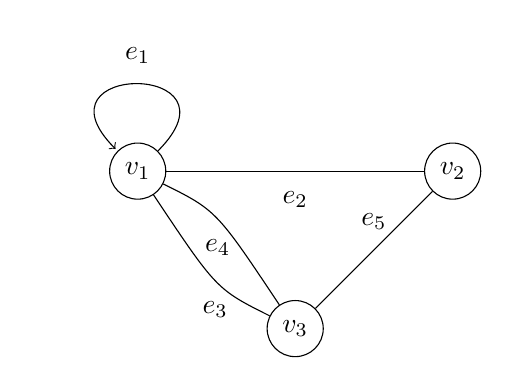
\begin{tikzpicture}
[scale=2,auto=left,every node/.style={circle}]
\node[circle,draw] (v1) at (0,0){$v_1$};
\node[circle,draw] (v2) at (2,0){$v_2$};
\node[circle,draw] (v3) at (1,-1){$v_3$};
\path  (v1)   edge[loop] node[above]  {$e_{1}$} (v1);
\draw (v1)--(v2)node[midway,below]{$e_2$};
\draw (v1)..controls(.5,-.75)..(v3)node[midway,below]{$e_3$};
\draw (v1)..controls(.5,-.25)..(v3)node[midway,below]{$e_4$};
\draw (v2) -- (v3) node[midway, above] {$e_5$};;
\end{tikzpicture}


Then the five walks of length 2 from $v_3$ to itself are.
\begin{eqnarray*}
v_3 e_5 v_2 e_5 v_3 & v_3 e_3 v_1 e_3 v_3\\
v_3 e_3 v_1 e_4 v_3 & v_3 e_4 v_1 e_4 v_3\\
v_3 e_4 v_1 e_4 v_3. & \\
\end{eqnarray*}

\end{document}